\section{State-sharing multi-observer}\label{ch:ssmo}
In this chapter, the state-sharing multi-observer (SSMO) will be discussed, aiming to reduce the required memory to store the CMO. The SSMO described in this chapter will provide the estimates as described in Subsection \ref{subsec:state-estimates} and will employ the same selection procedure as described in Subsection \ref{subsec:estimate-selection}.

\subsection{Constructing the state-estimates}
The SSMO follows the definition as in \cite{Chong2023MemoryAlgorithms}. Consider the observers
\begin{equation}\label{eqn:ssmo-observer}
    \begin{split}
        \dot{\hat{x}}^{\mcJ}_{j} &= \A_j^{\mcJ}\hat{x}^{\mcJ}_{j} - L_{j}^{\mcJ}C_{j}^{\mcJ}x + Bu -L_{j}^{\mcJ}(v_{j}^{\mcJ} + \tau_{j}^{\mcJ}), \quad \A_{j}^{\mcJ}=A+L_{j}^{\mcJ}C_{j}^{\mcJ} \\
        \dot{\hat{x}}_{p}^{\mcP} &= \A_p^{\mcP}\hat{x}_{p}^{\mcP} - L_{p}^{\mcP}C_{p}^{\mcP}x + Bu -L_{p}^{\mcP}(v_{p}^{\mcP} + \tau_{p}^{\mcP}), \quad \A_{p}^{\mcP}=A+L_{p}^{\mcP}C_{p}^{\mcP} \\
    \end{split}
\end{equation}
where $j=1,2,\dots,N_J$, $p=1,2,\dots,N_P$ with $N_J$ and $N_P$ as in Equation \eqref{eqn:multi-observer-sizes}. All $L$ must be selected in such a way that all $\A$ share the same characteristic polynomial
\begin{equation}\label{eqn:ssmo-char-poly}
    \det(sI-\A) = p(s) = s^n + q_1s^{n-1} + \dots + q_{n-1}s + q_n
\end{equation}
and thus all have equal eigenvalues. Let us now define a matrix $\Tilde{L}$ such that $\Tilde{L}y=Ly_{j}$ for all $J$-observers or $\Tilde{L}y=Ly_{p}$ for all $P$-observers. This can be achieved by padding $L$ with zero vectors $z \in \mathbb{R}^{n_x \times 1}$ \cite{Chong2023MemoryAlgorithms}. Let us now rewrite the observer \eqref{eqn:ssmo-observer} into the following form
\begin{equation}\label{eqn:ssmo-standard-system-form}
    \begin{split}
        \dot{\hat{x}}_{j}^{\mcJ} &= \A_{j}^{\mcJ}\hat{x}_{j}^{\mcJ} + \B_{j}^{\mcJ}\eta_{j}^{\mcJ}, \quad
        \B_{j}^{\mcJ} =
        \begin{bmatrix}
            B & -\Tilde{L}_{j}^{\mcJ} \\
        \end{bmatrix}, \quad \eta_j =
        \begin{bmatrix}
            u \\
            C_{j}^{\mcJ}x_{j}^{\mcJ} + v_{j}^{\mcJ} + \tau_{j}^{\mcJ}
        \end{bmatrix} \\ 
        \dot{\hat{x}}_{p}^{\mcP} &= \A_{p}^{\mcP}\hat{x}_{p}^{\mcP} + \B_{p}^{\mcP}\eta_{p}^{\mcP}, \quad
        \B_{p}^{\mcP} =
        \begin{bmatrix}
            B & -\Tilde{L}_{p}^{\mcP} \\
        \end{bmatrix}, \quad \eta_p =
        \begin{bmatrix}
            u \\
            C_{p}^{\mcP}x_{p}^{\mcP} + v_{p}^{\mcP} + \tau_{p}^{\mcP}
        \end{bmatrix}.
    \end{split}
\end{equation}

Let us now derive transformation matrices $T^{\mcJ}_{j}$ and $T_p^{\mcP}$ that transform all $\A^{\mcJ}_{j},\B^{\mcJ}_{j},\A^{\mcP}_{p}$ and $\B^{\mcP}_{p}$ as in \eqref{eqn:ssmo-standard-system-form} into controllable canonical form as in \cite[Sec. 4.3.2]{Hespanha2018LinearTheory}
\begin{equation}\label{eqn:controllable-canonical-form}
    \mathbf{A} =
    \begin{bmatrix}
        -q_1I_l & -q_2I_l & \cdots & -q_{n-1}I_l & -q_nI_l \\
        I_l & 0_l & \cdots & 0_l & 0_l \\
        0_l & I_l & \cdots & 0_l & 0_l \\
        \vdots & \vdots & \ddots & \vdots & \vdots \\
        0_l & 0_l & \cdots & I_l & 0_l \\
    \end{bmatrix}, \quad
    \mathbf{B} = 
    \begin{bmatrix}
        I_l \\ 0_l \\ \vdots \\ 0_l \\ 0_l \\
    \end{bmatrix}
\end{equation}
where $l=N$. The transformation matrices for each observer are,
\begin{equation}\label{eqn:ssmo-transformation}
    \begin{split}
        T_{j}^{\mcJ} &= R_j^{\mcJ}R_q \\
        T_{p}^{\mcP} &= R_p^{\mcP}R_q \\
        R_j^{\mcJ} &= 
        \begin{bmatrix}
            \B^{\mcJ}_{j} & \A^{\mcJ}_{j}\B^{\mcJ}_{j} & {(\A^{\mcJ}_{j})}^{2}\B^{\mcJ}_{j} & \cdots & {(\A^{\mcJ}_{j})}^{n-1}\B^{\mcJ}_{j} \\
        \end{bmatrix} \\
        R_p^{\mcP} &= 
        \begin{bmatrix}
            \B^{\mcP}_{p} & \A^{\mcP}_{p}\B^{\mcP}_{p} & {(\A^{\mcP}_{p})}^{2}\B^{\mcP}_{p} & \cdots & {(\A^{\mcP}_{p})}^{n-2}\B^{\mcP}_{p} \\
        \end{bmatrix} \\
        R_q &=
        \begin{bmatrix}
            I_l & q_1I_l & q_2I_l & \cdots & q_{n-1}I_l \\
            0_l & I_l & q_1I_l & \cdots & q_{n-2}I_l \\
            \vdots & \ddots & \ddots & \ddots & \vdots \\
            0_l & \cdots & 0_l & I_l & q_1I_l \\
            0_l & \cdots & 0_l & 0_l & I_l \\
        \end{bmatrix}.
    \end{split}
\end{equation}
The calculation showing that this transformation holds can be found in \autoref{ap:ssmo-transformation-matrix}. It should be noted that $\mathbf{A}$ and $\mathbf{B}$ are independent of $j$ and $p$. Since all observers \eqref{eqn:ssmo-observer} share the same characteristic polynomial \eqref{eqn:ssmo-char-poly}, $\mathbf{A}$ and $\mathbf{B}$ are the same for all observers. This means that only one copy of the matrices needs to be stored and all state estimates $\hat{x}$ can be recovered using the transformation matrices $T^{\mcJ}_{j}$ and $T^{\mcP}_{p}$

\begin{equation*}
    \hat{x}_{j}^{\mcJ} = T_{j}^{\mcJ} z, \quad \hat{x}_{p}^{\mcP} = T_{p}^{\mcP} z
\end{equation*}
where $z$ is the shared state which is governed by the equation
\begin{equation}\label{eqn:ssmo-z}
    \dot{z} = \mathbf{A}z + \mathbf{B}\eta, \quad \eta = 
    \begin{bmatrix}
        u \\ Cx + v + \tau
    \end{bmatrix}.
\end{equation}
An important requirement is that all state estimates $\hat{x}^{\mcJ}_{j}$ and $\hat{x}^{\mcP}_p$ share the same initial condition $\hat{x}^{\mcJ}_{j}(0)=\hat{x}^{\mcP}_p(0)$ for all $j=1,2,\dots,N_J$ and $p=1,2,\dots,N_P$, for simplicity it will be chosen as $0$.

\begin{figure}[h]
    \centering
    \begin{tikzpicture}[
        node distance=1.5cm,
        block/.style={rectangle, draw=black!60, very thick, minimum size=7mm, text centered},
        ]
    
    % System Block
    \node (system) [block, text width=4cm] {System \\ $\dot{x}(t) = Ax(t) + Bu(t)$ \\ $y_i = C_ix + Du + \tau_i$\\$i=1,2,\dots,N_O$};
    
    % Outputs Block
    \node (outputs) [block, right=of system, text width=4cm] {Outputs and input \\ $y_1, y_2, \dots, y_{N_O}$ and $u$};

    \node (shared-state) [block, below=of outputs, text width=4cm] {Shared state \\ $\dot{z} = \mathbf{A}z + \mathbf{B}\eta, \quad \eta = \begin{bmatrix} u \\ y \end{bmatrix}$};
    
    % Observers Section
    \node (Jobservers) [block, below=of shared-state, xshift=4cm, text width=4cm] {$J$-Observers \\ $\hat{x}_j^{\mcJ} = T^{\mcJ}_{j}z$ \\ $j=1,2,\dots,N_J$};
    \node (Pobservers) [block, below=of shared-state, xshift=-4cm, text width=4cm] {$P$-Observers \\ $\hat{x}_p^{\mcP} = T^{\mcP}_{p}z$ \\ $p=1,2,\dots,N_P$};
    
    % Comparison Block
    \node (comparison) [block, below=of Jobservers, xshift=-4cm, text width=4cm] {Comparison \\ $\pi_j = \max_{p \subset j} |\hat{x}^{\mcJ}_j - \hat{x}^{\mcP}_p|$ \\ $\sigma = \arg \min \pi_{\mathcal{J}}$};
    
    % Final Estimate Block
    \node (finalestimate) [block, right=of comparison, text width=4cm] {Final Estimate \\ $\hat{x} = \hat{x}^{\mcJ}_\sigma$};
    
    % Arrows
    \draw [->] (system) -- (outputs);
    \draw [->] (outputs) -- (shared-state);
    \draw [->] (shared-state) -- (Jobservers);
    \draw [->] (shared-state) -- (Pobservers);
    \draw [->] (Jobservers) -- (comparison);
    \draw [->] (Pobservers) -- (comparison);
    \draw [->] (comparison) -- (finalestimate);
    
    \end{tikzpicture}
    \caption{State sharing multi-observer diagram}
    \label{fig:ssmo-diagram}
\end{figure}

\subsection{Observer architecture}\label{subsec:ssmo-architecture}
Let us now discuss the way an SSMO is actually implemented. The calculation of $z$ is straightforward, Equation \eqref{eqn:ssmo-z} is used. the state estimates $\hat{x}^{\mcJ}_{p}$ and $\hat{x}^{\mcP}_p$ are calculated with the transformation matrices as follows

\begin{equation*}
    \tilde{x}_{SSMO} = \texttt{pm}(T,z,3),
\end{equation*}
where
\begin{center}
    % \begin{minipage}[t]{0.4\textwidth}
    %     \centering
    %     % first tikzpicture
    %     \begin{equation*}
    %         \begin{tikzpicture}[every node/.style={anchor=north east,fill=white,minimum width=1.2cm,minimum height=7mm}]
            
    %         % Define the displacement as a coordinate
    %         \coordinate (displacement) at (0.9,0.2);
        
    %         \matrix (mLP) [draw,matrix of math nodes]
    %             {
    %             \hat{x}_{\cP}^\mcJ \\
    %             };
        
    %         \matrix (dots2) [draw,matrix of math nodes] at ($(mLP.south west)+(displacement)$)
    %             {
    %             \dots \\
    %             };
        
    %         \matrix (mLp) [draw,matrix of math nodes] at ($(dots2.south west)+(displacement)$)
    %             {
    %             \hat{x}_{1}^\mcP \\
    %             };
        
    %         \matrix (mLJ) [draw,matrix of math nodes] at ($(mLp.south west)+(displacement)$)
    %             {
    %             \hat{x}_{\cJ}^\mcJ \\
    %             };
        
    %         \matrix (dots1) [draw,matrix of math nodes] at ($(mLJ.south west)+(displacement)$)
    %             {
    %             \dots \\
    %             };
        
    %         \matrix (mLj) [draw,matrix of math nodes] at ($(dots1.south west)+(displacement)$)
    %             {
    %             \hat{x}_1^\mcJ \\
    %             };
            
    %         \draw[dashed](mLj.north east)--(mLP.north east);
    %         \draw[dashed](mLj.north west)--(mLP.north west);
    %         \draw[dashed](mLj.south east)--(mLP.south east);
            
    %         \node at ($(-4,-1.8)$) {$\hat{x}_{SSMO}=$};
            
    %         \end{tikzpicture}
    %     \end{equation*}
    % \end{minipage}
    \begin{minipage}[t]{0.4\textwidth}
    \centering
    % Second tikzpicture
        \begin{equation*}\label{eqn:T-ssmo}
            \begin{tikzpicture}[every node/.style={anchor=north east,fill=white,minimum width=2cm,minimum height=7mm}]
            
            % Define the displacement as a coordinate
            \coordinate (displacement) at (1.7,0.2);
        
            \matrix (mLP) [draw,matrix of math nodes]
                {
                T^\mcP_{N_P} \\
                };
        
            \matrix (dots2) [draw,matrix of math nodes] at ($(mLP.south west)+(displacement)$)
                {
                \dots \\
                };
        
            \matrix (mLp) [draw,matrix of math nodes] at ($(dots2.south west)+(displacement)$)
                {
                T^\mcP_{1} \\
                };
        
            \matrix (mLJ) [draw,matrix of math nodes] at ($(mLp.south west)+(displacement)$)
                {
                T^\mcJ_{N_J} \\
                };
        
            \matrix (dots1) [draw,matrix of math nodes] at ($(mLJ.south west)+(displacement)$)
                {
                \dots \\
                };
        
            \matrix (mLj) [draw,matrix of math nodes] at ($(dots1.south west)+(displacement)$)
                {
                T^\mcJ_1 \\
                };

            
            \draw[dashed](mLj.north east)--(mLP.north east);
            \draw[dashed](mLj.north west)--(mLP.north west);
            \draw[dashed](mLj.south east)--(mLP.south east);
            
            \node at ($(-4,-1.8)$) {$T=$};
            
            \end{tikzpicture}
        \end{equation*}
    \end{minipage}
\end{center}
The structure of the storage matrix $\tilde{x}_{SSMO}$ is the same as $\tilde{x}_{3D}$ in Equation \eqref{eqn:A-tilde-3D}. The selection of the final estimate follows the same procedure as described in Section \ref{subsec:estimate-selection}.

\begin{table}[H]
    \centering
    \begin{tabular}{|c|c|c|}
        \toprule
       Matrix  & Dimensions & Number of elements \\ \midrule
       $\Tilde{x}_{SSMO}$  & $ n_x \times 1 \times N_S$ & $n_xN_S$ \\
       $\mathbf{A}$ & $n_xN_O \times n_xN_O$ & $n_x^2N_O^2$ \\ 
       $\mathbf{B}$ & $n_xN_O \times n_x$ & $n_x^2N_O$ \\
       $T$ & $n_x \times n_xN_O \times N_S$ & $n_x^2N_ON_S$ \\
       \bottomrule
    \end{tabular}
    \caption{SSMO system matrix dimensions}
    \label{tab:SSMO-dimensions}
\end{table}

\subsection{Size comparison}\label{subsec:size-comparison}
Let us now compare the sizes of the 2D-CMO, 3D-CMO and SSMO as presented in Tables \ref{tab:2D-CMO-dimensions}, \ref{tab:3D-CMO-dimensions} and \ref{tab:SSMO-dimensions} respectively. First, the total number of elements for each MO is derived from the matrices that are needed to construct it. 
\begin{table}[ht]
    \centering
    \begin{tabular}{|c|c|}
        \toprule
        Multi-Observer & Total number of Elements \\
        \midrule
        2D-CMO & $n_xN_S + n_x^2N_S^2 + n_xn_uN_S + n_u$ \\
        3D-CMO & $n_xN_S + 2n_x^2N_S$ \\
        SSMO   & $n_xN_S + n_x^2N_O^2 + n_x^2N_O + n_x^2N_ON_S$ \\
        \bottomrule
    \end{tabular}
    \caption{Total number of elements in each MO implementation}
    \label{tab:all-sizes}
\end{table}

We now use the for $N_S$ as in equation \eqref{eqn:NS-approximation} to compare number of Gigabytes required to store the MO. This value is derived from the number of elements, each element requires 8 bytes to be stored in for example a python float or a Matlab double. The comparison is made for different combinations of the number of state variables $n_x$ and number of total system outputs $N_O$. Both of these values are taken as $n \in \{1,2,\dots,50\}$ and the storage size for all $50^2=2500$ combinations are compared.

Figure \ref{fig:MO-storage}, where the colour indicates the total size of the MO, shows the result of this comparison. The 2D-CMO performs very poorly, as to be expected due to the $N_S^2$ term appearing in it's $A$ matrix (see \autoref{tab:2D-CMO-dimensions}). The 3D-CMO and the SSMO perform similarly. The size of all MOs increases much more with an increasing $N_O$ as compared to a growing $n_x$, which is not strange considering $N_O$ influences the number of combinations that need to be made from all sensors.
\begin{figure}[H]
    \centering
    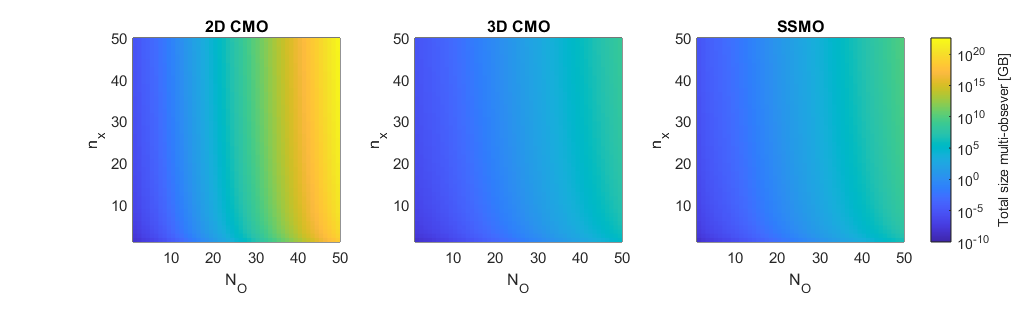
\includegraphics[width=\linewidth]{report/Figures/sizeComparison60.png}
    \caption{Storage requirements for different MOs}
    \label{fig:MO-storage}
\end{figure}
In Figure \ref{fig:ssmo-vs-3dcmo} the SSMO size is divided by the 3D CMO size, the plot shows the ratio between the two MOs. The figure clearly shows that the 3D CMO uses less memory than the SSMO under every circumstance. The difference becomes more pronounced for larger values of $N_O$. This can be attributed to the size of the $T$ matrix in Equation \ref{eqn:T-ssmo}, where its size $n_x^2N_ON_S$ can be viewed as $n_x^3N_S$ on the diagonal in Figure \eqref{fig:ssmo-vs-3dcmo}.
\begin{figure}[H]
    \centering
    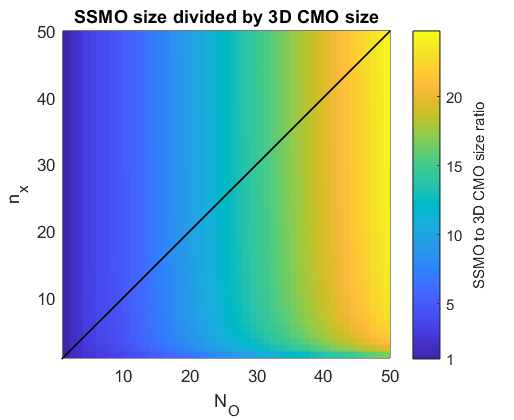
\includegraphics[width=0.4\linewidth]{report/Figures/ssmo_vs_3dcmo.png}
    \caption{Ratio between the required memory for an SSMO and 3D CMO respectively}
    \label{fig:ssmo-vs-3dcmo}
\end{figure}
It should also be noted that none of the MOs can be implemented in scenarios with a large $N_O$, since the required memory is significantly too large. Even the super computer Frontier with 9.6 Petabytes ($10^6$ Gigabytes) of random access memory would not be able to run such an MO \cite{2024FrontierDocumentation}. The calculations and plots shown in this subsection have been made with the Matlab script in Appendix \ref{ap:matlab-code-ch6}. The values in Figures \ref{fig:MO-storage} and \ref{fig:ssmo-vs-3dcmo} are all calculated with $P=1$, different values of $P$ could cause vastly different results if $P$ is chosen to be large. The relative size difference between the different MOs should stay similar.